\chapter{}
Os meses foram passando e logo outra novidade apareceu: Serra Pelada desencadeou uma verdadeira febre do ouro no Pará e garimpos apareciam por toda a região.
Todo mundo tinha em algum deles uma ``chupadeira'', nome que se dava ao equipamento empregado para ``chupar'' das barrancas dos rios o ouro de aluvião.
Não demorou muito e Zezão convidou o Paulo para se associar a ele na aquisição de quatro máquinas dessas.
Um terceiro sócio, um garimpeiro chamado Zezinho, entraria com o trabalho de exploração de duas lavras na região do Cumaru, um garimpo autorizado e supervisionado pela Polícia Federal.
O empreendimento chegou a render até um quilo de ouro por mês e uma rápida, mas fascinante incursão no universo do garimpo.
Através do que Paulo me contava, tomei contato com a estranha natureza daqueles homens que se internavam no meio do mato, longe de casa e da família por meses a fio, escavando toneladas de barro num trabalho de párias, para conseguir, ao fim de um dia extenuante, o equivalente a uma colherinha de café de minúsculas pepitas.
Capazes de persistir nesse esforço sobre-humano por dias e dias, anos e anos, pelo sonho de ``bamburrar'', isto é, de serem contemplados pelo milagroso encontro de uma grande pepita.
E que muitas vezes, ao serem abençoados dessa maneira, esbanjavam em poucas horas a dinheirama obtida, na satisfação de desejos quase infantis de ter e poder, quase sempre reprimidos ao longo de toda uma vida de miséria e privações.
Homens, que apesar disso tudo, demonstravam serem capazes de se pautar por um rígido código de decência na relação com seus companheiros de trabalho, se não por questão de honra ou lealdade, mas principalmente por necessidade de sobrevivência.
Naquela diminuta equipe que tocava o serviço de cada lavra, uns dependiam vitalmente dos outros e, por isso, não podia haver vacilo nem trapaça de espécie alguma.

\begin{figure}
\centering
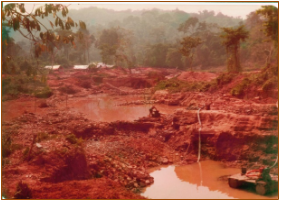
\includegraphics[width=0.7\linewidth]{32/garimpo-1.png}
\end{figure}

\begin{figure}
\centering
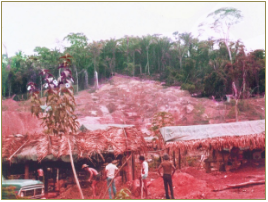
\includegraphics[width=0.7\linewidth]{32/garimpo-2.png}
\caption{O garimpo}
\end{figure}

Se por um algum tempo assaltara-me a angústia de que o sustento nos faltasse naquela terra tão distante, esse medo não tinha mais razão de ser.
Quando Paulo remetia de lá o dinheiro apurado mensalmente, a agência bancária do lugar reservava um horário especial para me atender.
Um dia, meu irmão Reginaldo, de passagem por Conceição para nos visitar, presenciou a chegada de uma remessa dessas.
Apavorado, correu a trancar portas e janelas, de medo de que alguém vendo aquilo nos atacasse.
Aquela generosa poupança nos serviria muito, mais adiante.

O temporário remanso em que entrou nossa vida permitiu-me olhar um pouco mais para mim mesma.
Sonhos recorrentes e facilmente identificáveis como ligados a perda de identidade começaram a povoar minhas noites.
Vez por outra alternavam-se com sonhos de morte em que eu me reconhecia na figura do agonizante.
Eu dera as costas ao meu trabalho e a uma condição de proteção e segurança que eu pouco ou nada precisara fazer para conquistar, além de usar o nome Filpi.
Agora, eu era Teresa, a mulher do Paulo, a mãe dos meninos e mais nada.
Estava, na imagem expressiva da sabedoria rabínica, ``acampada de frente para o mar''.
Havia uma ``terra prometida'' a procurar, uma passagem a enfrentar, uma nova identidade a construir.
Eu rompera não só com uma vida que ficou para trás, mas com uma imagem forjada desde a infância pelas expectativas familiares, de uma criatura sensata, adequada, sempre leal à causa da preservação do clã.
Minha decisão de partir de Araraquara no momento em que mamãe e meus irmãos se digladiavam na crise provocada pela morte do meu pai fora uma traição a esse passado, eu tinha certeza.


\textit{``Acampar em frente ao mar nos coloca num lugar de angústia e desconforto a partir do qual olhamos o horizonte''}, ensina um rabino que eu gosto de ler.
\textit{``Chegar até ele não é mais um processo do corpo, mas da alma.''} Intuindo confusamente o significado das minhas percepções, escrevi para Bel, minha cunhada psicóloga, mulher do João, contando-lhe o que se passava.
Respondeu-me aconselhando algumas leituras.
À distância, era tudo o que podia fazer para me ajudar.
Comecei, a partir dali, sozinha e com muito medo, um lento trabalho de desconstrução e reconstrução dos meus valores, das minhas crenças, da minha visão do mundo e de mim mesma.
\textit{``Nenhum acampamento''}, adverte ainda o meu rabino, \textit{``representa o futuro e a saída; todos eles são variações sobre a hesitação e a vacilação; são, na realidade, a fronteira onde um corpo morre para renascer com uma mesma alma em outro corpo, do outro lado da margem.''} 
Eu tinha que começar minha difícil travessia.
Só não sabia ainda que \textit{``achar-se é um perpétuo construir de identidades e desfazer-se delas em cada acampamento, à vista dos muitos horizontes que se propõem a nós ao longo da caminhada, à margem dos muitos mares que sempre nos separarão da outra margem.''}

Inocentemente alheios aos meus dramas de crescimento, as crianças cuidavam alegremente do seu próprio.
Era fantástico observar o que exprimiam nos seus desenhos e cartas.
Dona Yolanda, Marina e a própria Bel comentavam encantadas a riqueza do imaginário que a exuberante natureza à nossa volta ia esculpindo naquelas cabecinhas.
Fernando delirava nas cores, Marcelo nas formas.
Tomaz, racional e contido absorvia, impregnava-se de um profundo senso de autodeterminação que, um dia perceberíamos, tinha suas raízes naquela liberdade de uma infância vivida em plenitude.
Paula, única menina, teve que conquistar respeito no grito.
Risonha e alegre, virava bicho quando se sentia menos considerada.
Alfabetizou-se precocemente porque não admitia ficar à parte enquanto eu ensinava os mais velhos.
E que não lhe dessem atividade diferente a pretexto de que frequentava ainda a pré-escola.
Queria fazer o que os irmãos faziam.
Sem tirar nem por.
Vicente também não parecia contente na condição de caçula.
\textit{``Paula é metida a mandar''}, queixava-se ele.
A todo momento, com o arzinho professoral que é até hoje uma característica dela, queria dar um rumo aos rabiscos que, todo concentrado, o menorzinho ia desenhando sobre o papel, convicto de estar, ele também, cumprindo uma importante obrigação.
Era preciso um bocado de inventividade para mantê-los todos ocupados.
Mas aceitavam com tranquilidade aquelas horas extras de estudo e trabalhar com eles foi uma experiência que muito me ajudou quando um dia, por fim, retomei minha carreira.

Aos poucos, foi-me vindo a certeza de que ao menos no tocante à educação das crianças, estávamos no rumo certo.
Paulo, felizmente, compensava muito alguns aspectos que a minha educação tornara deficientes.
Com ele, as crianças aprenderam a enfrentar riscos, responsabilizando-se pela própria integridade física.
Fazia-se acompanhar por eles, sempre que possível, e estimulava-os a usufruir com naturalidade e prazer o contato com aspectos tão diversos da nossa terra, da nossa gente e da nossa cultura.
Acho que nisso está um dos diferenciais importantes que tornaram nossos filhos tão à vontade no mundo, tão tranquilos em lidar com situações novas e desafios, hoje em dia.


Nós os levávamos a viajar com certa frequência e a humilde Conceição acabou por proporcionar-lhes uma educação humanizada, o mais próximo da \textit{cura personalis} a que se poderia chegar.
A atenção pessoal dos professores, a afetividade daquela gente simples e espontânea, a convivência igualitária com os colegas da escola, da rua, do bairro, fizeram pelos meus filhos, eu suspeito, mais do que a leitura e discussão de teorias sociais e antropológicas em escolas de elite fariam.
Desfrutaram até o luxo de uma educação física aprimorada, não só pelas divertidas aulas de ginástica na coroa do Araguaia como pelo trabalho abnegado da jovem Wanda, uma excelente professora de natação que durante todo tempo em que lá permanecemos, sem esmorecer, soube manter aceso no seu diminuto grupo de pequenos atletas, um grande entusiasmo pela prática do esporte.

\begin{figure}
\hfill
\centering
\begin{subfigure}[h]{0.48\linewidth}
\centering
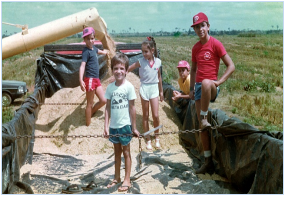
\includegraphics[width=\linewidth]{32/colheita-de-arroz.png}
\caption{Colheita de arroz na Nazaré.}
\end{subfigure}
\hfill
\begin{subfigure}[h]{0.48\linewidth}
\centering
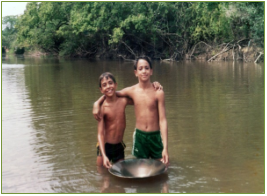
\includegraphics[width=1\linewidth]{32/bateia.png}
\caption{Brincando na bateia.}
\end{subfigure}
\end{figure}

\begin{figure}\ContinuedFloat
\hfill
\centering
\begin{subfigure}[h]{0.48\linewidth}
\centering
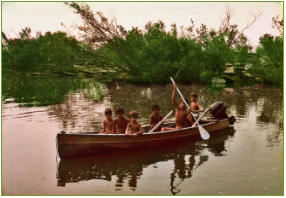
\includegraphics[width=\linewidth]{32/remando.png}
\caption{Remando nas águas do Curral de Pedra.}
\end{subfigure}
\hfill
\begin{subfigure}[h]{0.48\linewidth}
\centering
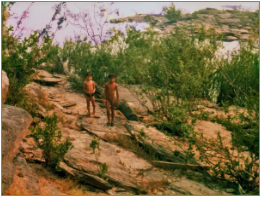
\includegraphics[width=1\linewidth]{32/passeando-curral.png}
\caption{Passeando no Curral de Pedra}
\end{subfigure}
\end{figure}

\begin{figure}\ContinuedFloat
\hfill
\centering
\begin{subfigure}[h]{0.48\linewidth}
\centering
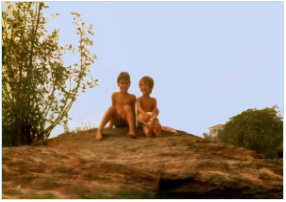
\includegraphics[width=\linewidth]{32/fernando+vicente.png}
\caption{Fernando e Vicente.}
\end{subfigure}
\hfill
\begin{subfigure}[h]{0.48\linewidth}
\centering
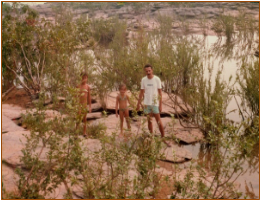
\includegraphics[width=1\linewidth]{32/paula+fernando+paulo.png}
\caption{Paula e Fernando com Paulo.}
\end{subfigure}
\end{figure}

\begin{figure}\ContinuedFloat
\hfill
\centering
\begin{subfigure}[h]{0.48\linewidth}
\centering
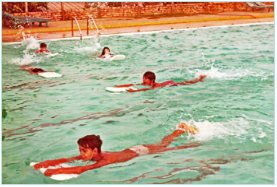
\includegraphics[width=\linewidth]{32/treinando.png}
\caption{Treinando no Clube.}
\end{subfigure}
\hfill
\begin{subfigure}[h]{0.48\linewidth}
\centering
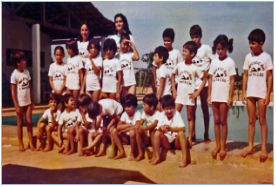
\includegraphics[width=1\linewidth]{32/turma-wandinha.png}
\caption{A turma de natação da Wandinha.}
\end{subfigure}
\end{figure}

\begin{figure}\ContinuedFloat
\hfill
\centering
\begin{subfigure}[h]{0.48\linewidth}
\centering
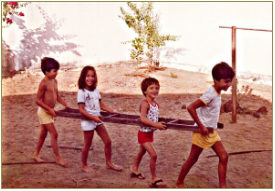
\includegraphics[width=\linewidth]{32/no-quintal.png}
\caption{Brincando no quintal de casa.}
\end{subfigure}
\hfill
\begin{subfigure}[h]{0.48\linewidth}
\centering
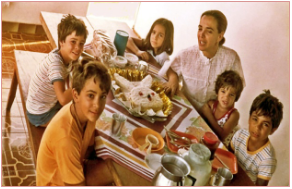
\includegraphics[width=1\linewidth]{32/páscoa.png}
\caption{Dia da Páscoa em Conceição.}
\end{subfigure}
\end{figure}

\begin{figure}\ContinuedFloat
\hfill
\centering
\begin{subfigure}[h]{0.48\linewidth}
\centering
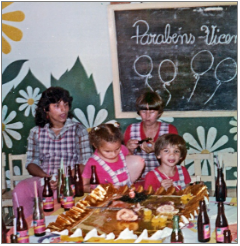
\includegraphics[width=\linewidth]{32/niver-vicente-sossego.png}
\caption{Aniversário do Vicente no Sossego de Mamãe.}
\end{subfigure}
\hfill
\begin{subfigure}[h]{0.48\linewidth}
\centering
\includegraphics[width=1\linewidth]{32/palhaço-botafogo.png}
\caption{O palhaço Botafogo.}
\end{subfigure}
\end{figure}

Entretanto, quando voltávamos periodicamente a São Paulo, ficava cada vez mais claro que os cinco se desenvolviam numa direção diametralmente oposta à das primas.
Não usavam tênis de marca, nem roupas de grife, nem sabiam o que era uma ``balada'' e mesmo quando descobriram, não se interessaram.
Gostavam de ler, aprendiam com facilidade e nunca viram a escola como suplício.
Nenhum dos ídolos e modismos que faziam delirar os primos parecia ter para eles o menor significado.
\textit{``Seus filhos não parecem desse mundo''}, me diziam.
\textit{``Vão ter dificuldade em se integrar à civilização quando voltarem para cá''}.
Nunca me deixei abalar por tais julgamentos, embora, se pudesse, preferisse poupá-los da chateação de lidar com o preconceito visível na expressão de alguns parentes.
Mas tinha que confiar em que saberiam se defender.
A situação não deixava de ser irritante, porque não havia outra saída a não ser ouvir e calar.
Contestar seria inútil.
Eu conhecia de sobra o desvertebrado produto da educação calcada no consumismo desvairado, na permissividade desenfreada e em falsos conceitos de contemporaneidade.
Como me opor a irmãos e cunhados tão convencidos das vantagens de aderir ao \textit{laissez-faire} pedagógico imperante, capaz de alinhar democraticamente pais e filhos no doce limbo de uma eterna adolescência? Limitei-me a colher, pacientemente, um importante material que alimentaria parte do meu trabalho com pais no dia em que me tornei coordenadora do colégio jesuíta de Teresina.

A educação das crianças era, porém, a única coisa sobre a qual eu me sentia segura.
No restante, a situação de ficar como apêndice do Paulo não me era confortável, mas eu não estava conseguindo enxergar outra possibilidade.
Ali, em Conceição do Araguaia, não via o que eu pudesse fazer para desenvolver um projeto pessoal e ganhar meu próprio dinheiro.
Paulo não entendia minha angústia.
Até porque, na sua crônica insegurança, ele nunca conseguiu aceitar minha necessidade de individualidade que ele confundia e ainda confunde com individualismo e falta de confiança nele.
Em aspectos periféricos até tolerava alguma independência desde que, no principal, professasse incondicional adesão às suas ideias e iniciativas.
Arregaçando as mangas e trabalhando com ele, nos projetos dele.
Não, eu não podia contar com o Paulo; já sabia de antemão que nesse percurso, ao contrário, eu o teria a maior parte do tempo, contra mim.

